\section{Unscented Kalman Filter}
In Kalman Filter, there are two important models, 
\begin{itemize}
\item Internal state model: $\mathbf{x}_t = f(\mathbf{x}_{t-1}, \mathbf{w}_{t-1})$
\item Observation model: $\mathbf{z}_t = h(\mathbf{x}_t, \mathbf{v}_t)$
\end{itemize}
where $\mathbf{x}_t$ and $\mathbf{z}_t$ are the internal state and the observation,
$\mathbf{w}_t$ and $\mathbf{v}_t$ are the process and measurement noise at time $t$, 
and both $f(\cdot)$ and $h(\cdot)$ are assumed linear. 
However, in many cases, at least one of the linear models does not hold. Therefore, methods for Kalman Filter with nonlinear model are proposed, including \gls{ekf} \cite{julier1997new} and \gls{ukf} \cite{wan2000unscented}. 
\gls{ekf} uses Taylor series expansion to approximate the nonlinearity, may introduce errors for the true mean and covariance of the state variables after the non-linear transformation.
Additionally, in our case, there is no close-formed nonlinear motion model under camera projection. 
Consequently, we use \gls{ukf}, where its nonlinear state model $f(\cdot)$ is learned by the non-parametric model \gls{gp}.

\begin{figure}
\centering
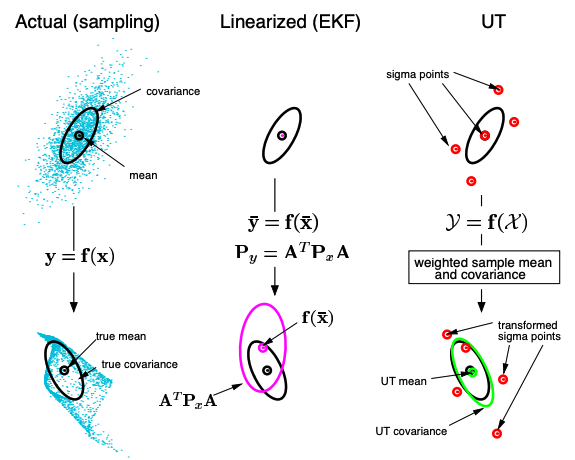
\includegraphics[width=\linewidth]{./img/gp/ut.png}
\caption{Example of the UT for mean and covariance propagation. a) actual, b) first-order linearization (EKF), c) UT.}
\label{fig:ufk-ut}
\end{figure}

The key of \gls{ukf} is \gls{ut}, which calculates the statistics of random variables under a nonlinear transformation, accurately capturing the mean and the covariance to the 3rd order Taylor series expansion for Gaussian inputs. 
For a random variable $\mathbf{x} \in \mathbb{R}^{d}$ with mean $\bar{\mathbf{x}}$ and covariance $\mathbf{P_x}$, to calculate the statistics of $\mathbf{z}$ under a nonlinear mapping $\mathbf{z} = g(\mathbf{x})$, first a set of sigma points are built around the $\bar{\mathbf{x}}$ \cite{wan2000unscented},
\begin{align}
\begin{split}
\mathcal{X}_0 & = \bar{\mathbf{x}} \\
\mathcal{X}_i & = \bar{\mathbf{x}} + (\sqrt{(d+\lambda)\mathbf{P_x}})_i, \qquad i = 1, \dots, d\\
\mathcal{X}_i & = \bar{\mathbf{x}} - (\sqrt{(d+\lambda)\mathbf{P_x}})_i, \qquad i = d+1, \dots, 2d\\
W_0^{(m)} & = \lambda/(d+\lambda) \\
W_0^{(c)} & = \lambda/(d+\lambda) + (1-\alpha^2+\beta) \\
W_i^{(m)} & = W_i^{(c)} = 1/\{2(d+\lambda)\} \qquad i = 1, \dots, 2d
\end{split}
\end{align}

where $\alpha$ controls the spread of the sigma points around $\bar{\mathbf{x}}$, 
$\lambda = \alpha^{2}(d+\kappa)-d$ and $\kappa$ are the scaling parameters,
$\beta$ describe the prior knowledge for the distribution of $\mathbf{x}$.
$\alpha$ is usually set to a small value (\eg $1e-3$),
$\kappa$ is usually set to 0 and $\beta$ is optimally set to $2$ for Gaussian distribution.
$(\sqrt{(d+\lambda)\mathbf{P_x}})_i$ is the $i$th row of the matrix square root. 
Each sigma point is propagated through the nonlinear function $g(\cdot)$, 
$$\mathcal{Z}_{i} = g(\mathcal{X}_i) \qquad i = 0, 1, \dots, 2d,$$
The mean and covariance for $\mathbf{z}$ are approximated by the weighted sample mean and covariance of the posterior sigma points,
\begin{align}
\bar{\mathbf{z}} & \approx \sum_{i=0}^{2d}{W_i^{(m)}\mathcal{Z}_i}\\
\mathbf{P_z} & \approx \sum_{i=0}^{2d}{W_i^{(c)}(\mathcal{Z}_i-\bar{\mathbf{z}})(\mathcal{Z}_i-\bar{\mathbf{z}})^T}
\end{align}

Therefore, with the non-linear state and measurement model, \gls{ukf} naturally extends the unscented transformation by applying it alternately between the predict and correct step.